\chapter{有限元素法}

\begin{figure}[hbt!]
\begin{center}
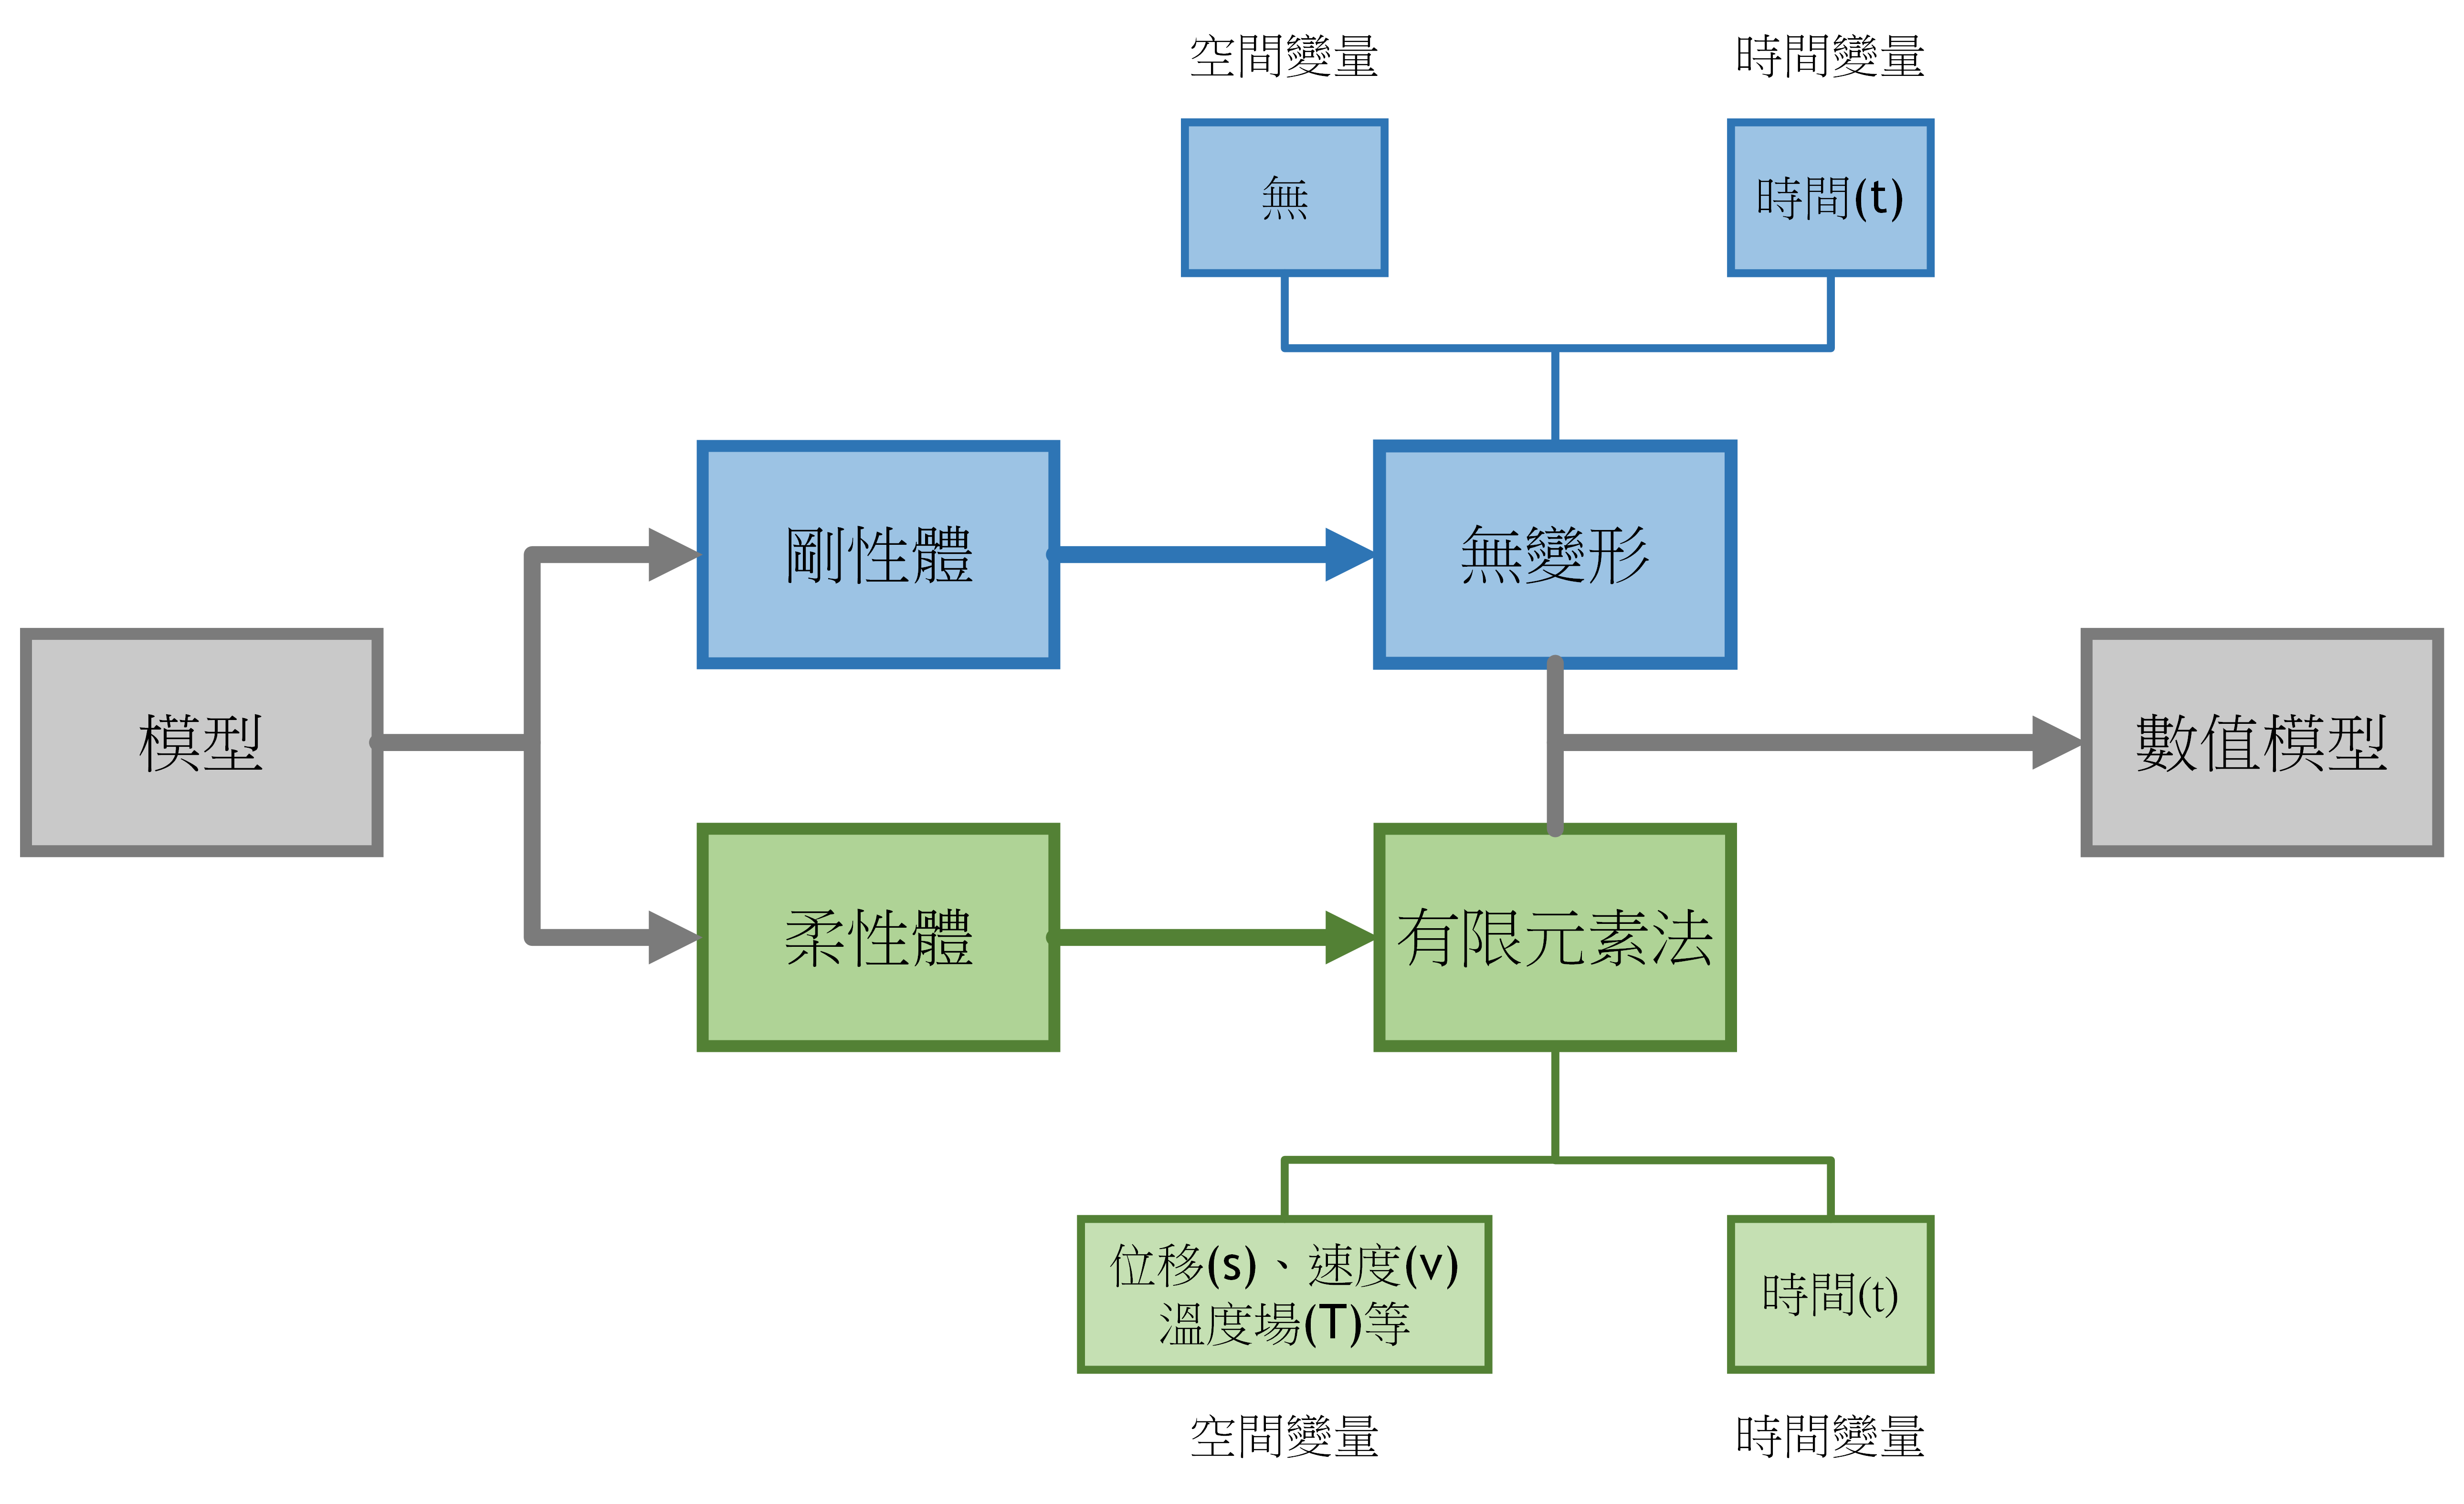
\includegraphics[width=15cm]{有限元素法}
\caption{\Large 有限元素法介紹}\label{有限元素法}
\end{center}
\end{figure}
時間及空間問題常用偏微分方程(PDE)做數值求解,將根據不同的模型進行弱化、離散化等求解,此動作稱為有限元素法(FEM),通過在模型上簡化連續變量的複雜性來實現近似求解,用於複雜的工程結構或物理系統的行為。\\

而柔性體則會因為受力情況的不同而產生多種變量,才需要利用偏微分方程求解,對物體進行弱化、離散化並劃分網格如(圖 \ref{有限元素法}),接著代入方程計算,此動作稱為有限元素法。\\

因為可以對複雜模型進行分析,所以在近代被廣泛的使用,在機械、建築等領域都可以看到其身影。
\newpage
%---------------------第二章/基本概念及假設假定-------------------------%
\section{基本概念}


\begin{figure}[hbt!]
\begin{center}
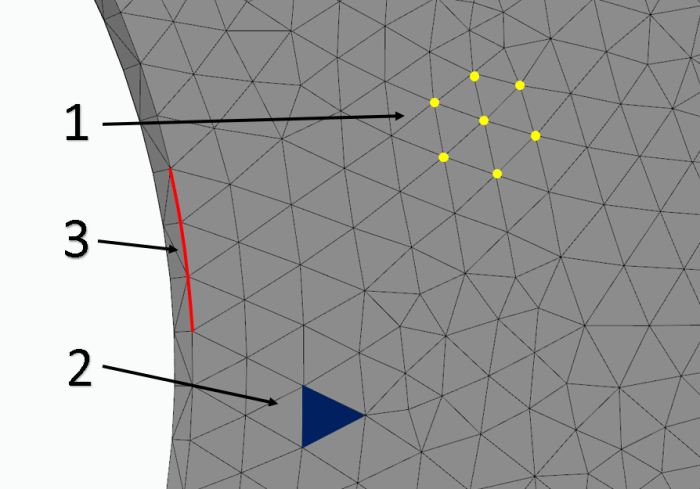
\includegraphics[width=12cm]{有限元素法介紹}
\caption{\Large 基本概念}\label{有限元素法介紹}
\end{center}
\end{figure}

\begin{enumerate}
\item 節點:每個元素的角落或中心點,用於連接元素之間的邊界條件和解決方程,如(圖 \ref{有限元素法介紹})上1指示。
\item 元素:通常由三角形或者四邊形等形成的區域結構,如(圖 \ref{有限元素法介紹})上2所示。
\item 邊界條件:存在於物理系統邊界如(圖 \ref{有限元素法介紹})上3所示的約束及負荷力,模擬實際情況下的條件約束和外界影響,。
\item 自由度: 節點上變量的個數,例如位移的節點自由度為3,表示單個節點擁有三個坐標方向的位移,又例如熱分析時節點自由度為1,表示某個節點處的溫度。
\item 網格:由數個元素經由節點連接所組成,表示在需分析的區域上。
\item 變形:邊界條件的影響下的形變,經過分析後計算每個元素的變形及變形之間的相互影響預測整得系統變化。
\item 離散化:將物理系統或結構等連續變量通過計算轉換為數格元素的過程,目的在於減化連續變量的複雜性,便於處理及分析。關於公式及步驟會因為模型或問題的類型不同而有不一樣的計算方式。
\item 材料特性:物理系統(模型)的材料性質,不同的材料其中的參數各為不同(彈性模數、蒲松比、極限強度、降伏強度等)。\\
\end{enumerate}

\subsection{邊界條件}
分為兩種邊界條件,為位移值或施加力條件。

\begin{enumerate}
\item 位移邊界條件:規定了結構或邊界上的位移及變形的特定值或關係。

\begin{itemize}
\item 固定邊界條件:也稱為約束邊界條件,令特定的某些節點或自由度的位移為零,使其無法發生位移。
\item 位移約束:指定特定節點或自由度的位移值, 可以是定值或隨時間變化的函數。
\item 斜率約束:規定特定節點的自由度的位移斜率(導數),用於描述特定邊界上的傾斜或旋轉。
\end{itemize}

\item 力邊界條件:規定了結構或邊界上施加的外部力或力的分布。

\begin{itemize}
\item 負荷:施加在結構上的集中力或分布力,可以是靜態或動態負荷。
\item 壓力:施加在邊界上的或表面力,可以是均勻或非均勻的。
\item 動力學條件:施加在結構上的動態加載。\\
\end{itemize}
\end{enumerate}

\subsection{網格劃分基本原則}

\begin{enumerate}
\item 網格數量:將決定計算精度及規模大小,一般狀況中,網格數量增加計算精度也會跟著提升,但伴隨而來的是更大的計算量,所以在制定網格大小時應權衡兩個因素。
\item 網格疏密:在某些變化梯度較大的部位(應力集中處),需要大密集的網格,密集往個將更好反映數據變化,反之變化梯度較小的部位則用較稀疏的網格,而不同單元之間的連接則採用特殊的過度單元或多點約束等方法連接,才能更好的分配資源,兼顧計算量何計算精度。
\item 網格質量:指網格形狀的合理性,質量的好壞將直接影響計算精度,質量較差的除了造成局部的計算精度偏差甚至會直接終止計算,因此在重要部位時應該確保其擁有高品質的表現,如果網格都是由等邊三角形、正方形、正四面體、立方六面體等組成,則求解精度可以非常接近實際值,但這種只存在於理想狀態下,實際運用卻很難做到。\\
\end{enumerate}

\begin{itemize}
\item 元素質量評價指標
\end{itemize}

\begin{enumerate}
\item 單元的邊長比、面積比及體積比,理想的邊長比為1,以正三角形、正四面體、正六面體為參考基準。
\item 扭曲度:單元內部扭轉及面外的翹曲程度。
\item 疏密過渡:應力梯度方向和橫向過渡情況,應力集中部分應較為密集,則反之。
\item 節點、元素排部:合理的節點及元素有助於帶入方程式計算,可以提高求解效率,並且須注意消除重複的節點及元素。
\end{enumerate}
下列(圖 \ref{網格1mm-1})至(圖 \ref{網格50mm-2})為網格疏密不同造成的分析差\

\begin{figure}[htbp]
  \centering
  \begin{minipage}{0.4\textwidth}
    \centering
    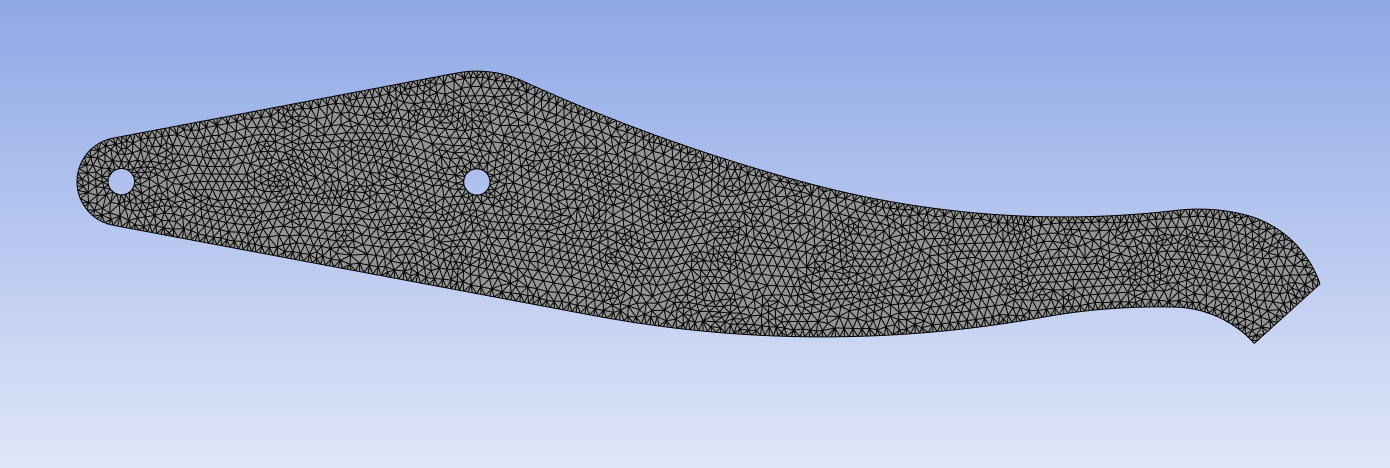
\includegraphics[width=\textwidth]{網格1mm-1}
    \caption{較密網格}
    \label{網格1mm-1}
  \end{minipage}
  \hfill
  \begin{minipage}{0.4\textwidth}
    \centering
    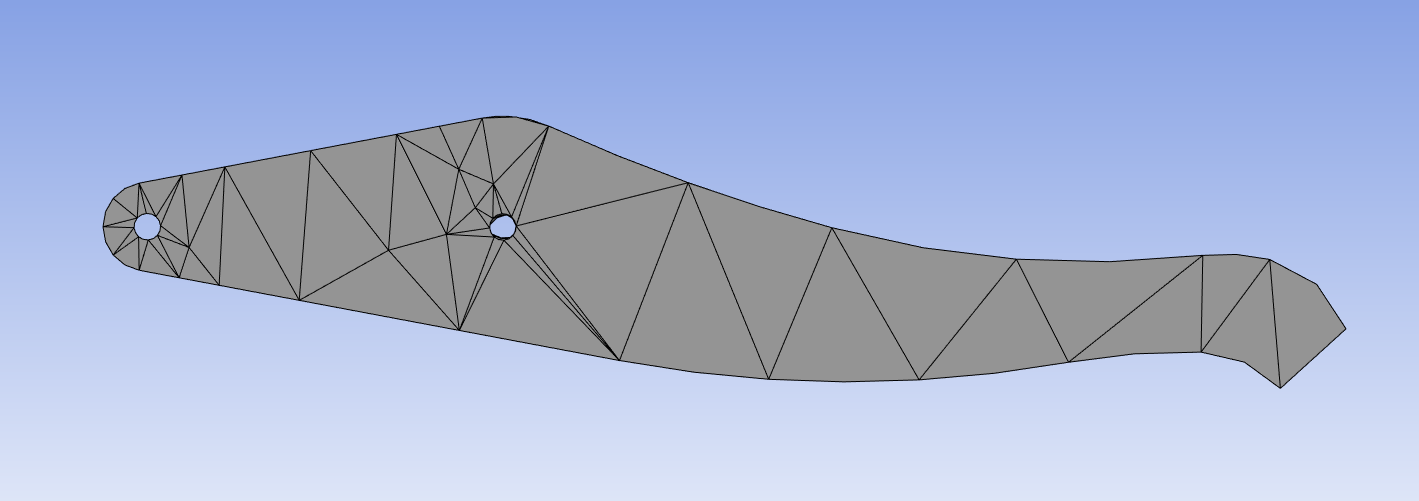
\includegraphics[width=\textwidth]{網格50mm-1}
    \caption{較粗網格}
    \label{網格1mm-2}
  \end{minipage}
  
  \begin{minipage}{0.4\textwidth}
    \centering
    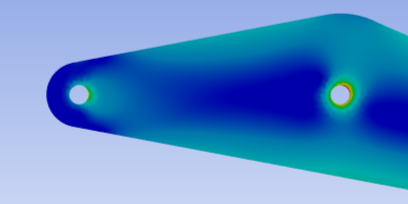
\includegraphics[width=\textwidth]{網格1mm-2}
    \caption{較密網格所得應力雲圖}
    \label{網格50mm-1}
  \end{minipage}
  \hfill
  \begin{minipage}{0.4\textwidth}
    \centering
    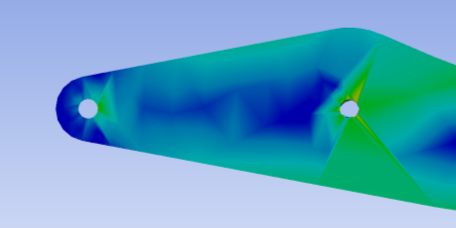
\includegraphics[width=\textwidth]{網格50mm-2}
    \caption{較粗網格所得應力雲圖}
    \label{網格50mm-2}
  \end{minipage}
\end{figure}
\newpage

%--------------------------第二章/有限元計算公式--------------------------%
\section{計算及公式介紹}
此章節主要介紹常見的結構力學的有限元計算公式及方法順序,了解到平時由電腦計算的有限元素法及代數方程式,觀察固體結構上變形及應力是如何進行分析計算以及選用原因。\\

\subsection{變形分析}

在有限元素分析中,通常使用格拉朗日公式,透過觀察材料的平移或旋轉來建立力學方程。
在材料上設置隨意點(X),觀察點(X)隨時間(t)變化後的材料位移矢量u(X,t),轉換為空間坐標系x=X+u即可以得到一個拉格朗日公式,只要材料為柔性體就會產生局部變化,此現象稱為應變或伸長,下列將透過多種方式來描述材料變形過程。\\

\begin{itemize}
\item 變形梯度
\end{itemize}

變形梯度F定義為
$$\mathbf{F}=\frac{\partial \mathbf{x}}{\partial \mathbf{X}}=\mathbf{I}+\frac{\partial \mathbf{u}}{\partial \mathbf{X}}$$\

其中, $\mathbf{I}$ 等同張量, 展開為矩陣形式為:\

$$\mathbf{F}=\left[\begin{array}{lll}
\frac{\partial x}{\partial X} & \frac{\partial x}{\partial Y} & \frac{\partial x}{\partial Z} \\
\frac{\partial y}{\partial X} & \frac{\partial y}{\partial Y} & \frac{\partial y}{\partial Z} \\
\frac{\partial z}{\partial X} & \frac{\partial z}{\partial Y} & \frac{\partial z}{\partial Z}
\end{array}\right]=\left[\begin{array}{ccc}
1+\frac{\partial u}{\partial X} & \frac{\partial u}{\partial Y} & \frac{\partial u}{\partial Z} \\
\frac{\partial v}{\partial X} & 1+\frac{\partial v}{\partial Y} & \frac{\partial v}{\partial Z} \\
\frac{\partial w}{\partial X} & \frac{\partial w}{\partial Y} & 1+\frac{\partial w}{\partial Z}
\end{array}\right]$$
\\

上述矩陣包含材料局部旋轉和變形的完整解釋,其中還顯示許多訊息,例如:\

由於dx=FdX,未變形體dX中小線段是如何旋轉並拉伸,成為變形體dX中的線段,我們將F張量看做一個矩陣,第一列提供線段最開始沿X方向的大小和方向等信息。從數學角度來看,F是從X改變到x雅可比矩陣,因此它的行列為式J=det(F)為局體體積比例因子,為不可壓縮材料$J=1$。\\

極分析定理表明,任何二階張量都可以分解為純轉動和對稱張量的成績,利用這一定理將剛體轉動與變形分開:\
$$F=R U$$

這可以解釋為先發生變形(伸長張量U),再進行剛性旋轉(旋轉矩陣R)。如此一來,如果沒有旋轉,右伸長張量則為變形梯度,因此U的解釋與F類似。\\

同樣也可以將變形梯度分解為\
$$F=V R$$

此過程中,會先發生剛體轉動,然後轉動的體發生形變,變形透過左伸長量(V)描述。\\

這兩個伸長張量($U$)、($V$)通過純轉向有著關聯,例如$\mathbf{V}=\mathbf{F R}^T=\mathbf{R} \mathbf{U} \mathbf{R}^T$。事實上此處旋轉矩陣的轉置也是自身的逆 $\left(\mathbf{R}^T \mathbf{R}=\mathbf{R R}^T=\mathbf{I}\right)$ 。\\

在實踐操作中,極分析的計算結果趨向於更高,因此,人們會盡量避免這種類型的計算。但在理論思考方面,這個概念非常有用。我們可以在不確定旋轉矩陣的情況下,計算與旋轉無關的變形測量:\
$$\mathbf{F}^T \mathbf{F}=(\mathbf{R U})^T \mathbf{R} \mathbf{U}=\mathbf{U}^T \mathbf{R}^T \mathbf{R} \mathbf{U}=\mathbf{U}^T \mathbf{U}=\mathbf{U}^2=\mathbf{C}$$

張量C稱為右柯西-格林變形張量。\\

這個張量經常用於描述超彈性材料的本構特性等,僅由U張量構成,因此用描述材料在旋轉“之前”的變形。\\

由此可知\
$$\mathbf{F} \mathbf{F}^T=\mathbf{V R}(\mathbf{V R})^T=\mathbf{V R R}^T \mathbf{V}^T=\mathbf{V} \mathbf{V}^T=\mathbf{V}^2=\mathbf{B}$$

$B$和$C$都與旋轉無關,但它們描述的是兩個不同坐標系中的變形。\\

張量$C$是描述材料坐標系中變形的材料張量,$B$是描述空間坐標系中變形的空間張量。\\

\begin{itemize}
\item 伸長率
\end{itemize}
從非正式意義上來說,伸長率可定義為當前長度與原始長度之比\
$$\lambda=\frac{L}{L_0}$$

因此在末變形狀態下,伸長率為1。一般情況下,人們更傾向於使用張量U和C的特徵值。U的三個特徵值$\left(\lambda_1\right)$、$\left(\lambda_2\right.$ 和 $\left.\lambda_3\right)$稱為主伸長率,其對應的特徵矢量在材料坐標系中給出三個正交方向。如果我們研究一個小立方體(正方體),其中三條邊沿著這三個方向,則它將會發生變化成為長方體,但所有邊仍保持直角相交。邊長變化由主伸長率表示。\
如此一來體積變化可以寫為主伸長率的乘積:\
$$\frac{V}{V_0}=\lambda_1 \lambda_2 \lambda_3$$\

張量C的計算更加簡單,它的主方向與U相同,但特徵值為$\lambda_1^2$、$\lambda_2^2$和$\lambda_3^2$。因此通常使用C而非U來計算主伸長率。\\

對於未變形材料(剛體)C=I。解釋了為甚麼在實際中人們主要使用C來描述較大伸縮性的材料。\\

左柯西-格林變形張量B也具有主伸長率作為特徵值。但由于V描述剛體轉動之後的伸長率,因此主方向依照空間方向來確定。\\

\begin{itemize}
\item 應變張量
\end{itemize}

要得到基于零的變形測量值,需要從C中減去等同張量,從而得到格林-拉格朗日應變張量E定義為\
$$\mathbf{E}=\frac{1}{2}(\mathbf{C}-\mathbf{I})$$

該張量也描述材料在發生任何轉動之前產生的變形,但在未變形狀態下的所有分項均為零,其分項可以寫為\
$$E_{i j}=\frac{1}{2}\left(\frac{\partial u_i}{\partial X_j}+\frac{\partial u_j}{\partial X_i}+\frac{\partial u_k}{\partial X_i} \frac{\partial u_k}{\partial X_j}\right)$$\

其中假設對重複指標求和。\\

格林-拉格朗日應編張量的對角元素如下\
$$E_{X X}=\frac{\partial u}{\partial X}+\frac{1}{2}\left(\left(\frac{\partial u}{\partial X}\right)^2+\left(\frac{\partial v}{\partial X}\right)^2+\left(\frac{\partial w}{\partial X}\right)^2\right)$$\

非對角元素的示例為\
$$E_{X Y}=\frac{1}{2}\left(\frac{\partial u}{\partial Y}+\frac{\partial v}{\partial X}+\frac{\partial u}{\partial X} \frac{\partial u}{\partial Y}+\frac{\partial v}{\partial X} \frac{\partial v}{\partial Y}+\frac{\partial w}{\partial X} \frac{\partial w}{\partial Y}\right)$$\

當應變和剛體轉動幅度都很小時,格林-拉格朗日應編張量中的二次項可以忽略不計,由此可得到工程應變張量\

$$\varepsilon_{i j}=\frac{1}{2}\left(\frac{\partial u_i}{\partial X_j}+\frac{\partial u_j}{\partial X_i}\right)$$\

其分量如下\
$$\varepsilon_{X X}=\frac{\partial u}{\partial X}$$\

和\
$$\varepsilon_{X Y}=\frac{1}{2}\left(\frac{\partial u}{\partial Y}+\frac{\partial v}{\partial X}\right)$$\

該應變張量的對角項稱為法向應變或正應變,用於描述沿每個坐標軸的延伸。非對角項是應變張量的剪切分量,用於描述線段之間夾角的變化。這裡的術語很容易被混淆,因為在工程領域,由於$\gamma_{i j}$直接測量角度的變化(以弧度表示),所以人們習慣使用“剪切應變”一詞來描述物理量$\gamma_{i j}=2 \varepsilon_{i j}=$
剪切應變產生等體積變形;即變形不引起體積改變。對於小應變相對體積變化通過正應變之和求得:\
$$\frac{\Delta V}{V}=\varepsilon_{x x}+\varepsilon_{y y}+\varepsilon_{z z}=\operatorname{trace}(\varepsilon)$$

\begin{itemize}
\item 真實應變
\end{itemize}

有時,我們會使用真實應變 這個術語。在真實應變的單軸定義中,應變增量定義為\
$$d \varepsilon=\frac{d L}{L}$$\

真實應變的定義基於當前長度,因此在積分後可以得到\
$$\varepsilon=\ln \left(\frac{L}{L_0}\right)=\ln (\lambda)$$\

這就是真實應變也稱為對數應變的原因。\\

\begin{itemize}
\item 應變協調性
\end{itemize}

由於應變張量由位移的導數構成,因此並非所有應變場均適用。位移矢量只有三個分量,這意味著,除非各個應變分量都滿足特定的協調性標準,否則它們的積分無法給出唯一的一組位移。工程應變必須滿足以下方程:\
$$\frac{\partial^2 \varepsilon_{i j}}{\partial X_k \partial X_l}+\frac{\partial^2 \varepsilon_{k l}}{\partial X_i \partial X_j}-\frac{\partial^2 \varepsilon_{i k}}{\partial X_j \partial X_l}-\frac{\partial^2 \varepsilon_{j l}}{\partial X_i \partial X_k}=0$$\

由於應變張量的對稱性,這81 個方程中只有6 個是非平凡方程。如下所示:\
$$
\begin{aligned}
\frac{\partial^2 \varepsilon_{x x}}{\partial y \partial z} & =\frac{\partial}{\partial x}\left(-\frac{\partial \varepsilon_{y z}}{\partial x}+\frac{\partial \varepsilon_{z x}}{\partial y}+\frac{\partial \varepsilon_{x y}}{\partial z}\right) \\
\frac{\partial^2 \varepsilon_{y y}}{\partial z \partial x} & =\frac{\partial}{\partial y}\left(-\frac{\partial \varepsilon_{z x}}{\partial y}+\frac{\partial \varepsilon_{x y}}{\partial z}+\frac{\partial \varepsilon_{y z}}{\partial x}\right) \\
\frac{\partial^2 \varepsilon_{z z}}{\partial x \partial y} & =\frac{\partial}{\partial z}\left(-\frac{\partial \varepsilon_{x y}}{\partial z}+\frac{\partial \varepsilon_{y z}}{\partial x}+\frac{\partial \varepsilon_{z x}}{\partial y}\right) \\
2 \frac{\partial^2 \varepsilon_{x y}}{\partial x \partial y} & =\frac{\partial^2 \varepsilon_{x x}}{\partial y^2}+\frac{\partial^2 \varepsilon_{y y}}{\partial x^2} \\
2 \frac{\partial^2 \varepsilon_{y z}}{\partial y \partial z} & =\frac{\partial^2 \varepsilon_{y y}}{\partial z^2}+\frac{\partial^2 \varepsilon_{z z}}{\partial y^2} \\
2 \frac{\partial^2 \varepsilon_{z x}}{\partial z \partial x} & =\frac{\partial^2 \varepsilon_{z z}}{\partial x^2}+\frac{\partial^2 \varepsilon_{x x}}{\partial z^2}
\end{aligned}
$$\

\subsection{應力方程}

\begin{itemize}
\item 動量平衡
\end{itemize}

作用在變形區域上的表面力可以表示為\
$$d \mathbf{F}_s=\mathbf{t}_n d a=\mathbf{T}_N d A$$\

其中$\mathbf{t}_{\mathrm{n}}$稱為牽引力,而 $\mathbf{T} \mathrm{N}$通常稱為標稱牽引力,原因是它將實際變形狀態下的作用力與未變形區域關聯起來。\\

此外,我們還可以基於法矢將牽引分量寫為以下線性展開式:\
$$T_i=P_{i J} N_J$$\

在此處和下文中,假設對重複指標求和。空間分量和材料分量分別使用小寫和大寫字母。這種表示有時稱為柯西定律或柯西公式,僅適用於$P_{i J}$為特定二階張量的分量的情況。對於任意未變形的材料體積$V_0$ ',動量守恆可以用以下積分形式表示:\
$$\frac{d}{d t} \int_{V_0} \rho_0 \mathbf{v} d V=\int_{V_0} \mathbf{f}_V d V+\int_{\partial V_0} \mathbf{T} d A$$\

其中$\mathbf{f}_V$ 表示體積力\\

速度場根據位移場 $\mathbf{u}$計算為\

$$\mathbf{v}=\frac{\partial \mathbf{u}}{\partial t}(\mathbf{X}, t)$$

根據散度定理,使用柯西公式可以將表面積分轉換為體積積分:\
$$\int_{\partial V_0} T_i d A=\int_{\partial V_0} P_{i J} N_J d A=\int_{V_0} \frac{\partial P_{i J}}{\partial X_J} d V$$\

因此可以得到動量平衡方程的微分形式如下所示:\
$$\rho_0 \frac{\partial^2 u_i}{\partial t^2}=f_{V, i}+\frac{\partial P_{i, J}}{\partial X_J}$$\

或者使用張量符號:\
$$\rho_0 \frac{\partial^2 \mathbf{u}}{\partial t^2}=\mathbf{f}_V+\nabla_X \cdot \mathbf{P}^{\mathbf{T}}$$\

張量P稱為第一類Piola-Kirchhoff應力張量,它將空間方向的作用力與原始未變形構型中的區域關聯起來。量指標涉及不同的構型。有時這種數學對象稱為兩點張量。\\

在實際的變形構型中,可以對牽引矢量$\mathrm{t}_{\mathrm{n}}$和材料體積應用類似的方法,可用下式表示:\
$$\mathbf{t}_n=\sigma_{i j} n_j \mathbf{e}_i$$\

張量$\sigma$ 稱為柯西應力張量或真實應力張量,原因是它表示與實際變形區域相關的實際構型中的力。由其空間分量表示。\\

由於柯西應力張量和第一類Piola-Kirchhoff 應力張量對同一個表面力有著不同的表示\
$$\mathbf{P N} d A=\sigma \mathbf{n} d a$$\

要確定這兩種應力測量方式之間的關係,我們可以使用Nanson公式 計算變形引起的面積變化,表示為\
$$\mathbf{n} d a=J \mathbf{F}^{-T} \mathbf{N} d A$$\

其中,F為變形梯度張量,由此可得\
$$J=\operatorname{det}(\mathbf{F})=d V / d V_0$$\

體積因子J可以給出變形引起的體積變化。因此,應力張量可通過下式與之關聯\
$$\mathbf{P}=J \sigma \mathbf{F}^{-T}$$\

通過引入一個稱為基爾霍夫應力張量(定義為$\tau=J \sigma$ )的張量,可以進一步簡化這個公式及類似公式。基爾霍夫應力張量是一個幾乎沒有實際用途的物理量,但卻具有理論上的便利性。\\

\begin{itemize}
\item 機械能平衡
\end{itemize}

將動量方程的微分形式乘以速度矢量,並基於材料對其進行積分,可以得到以下方程:\
$$\frac{d}{d t} \int_V \frac{1}{2} \rho v^2 d V+\int_V \sigma: \mathbf{L} d V=\int_V \mathbf{f}_v \cdot \mathbf{v} d V+\int_{\partial V} \mathbf{t}_n \cdot \mathbf{v} d A$$\

這個方程給出了機械能平衡的積分形式,也稱為冪定理。速度的空間梯度為$\mathbf{L}=\nabla_x \mathbf{V}$,其中的運算符表示對兩個指標求和\
$$\int_V \sigma: \mathbf{L} d V=\int_{V_0} \mathbf{P}: \dot{\mathbf{F}} d V_0$$\

變形分析頁面對速度梯度的特性進行了詳細論述。\\

方程右側的兩個積分項分別表示體積力和表面力的功率輸入,它們分別是這些力在每單位時間內對材料所做的功。左側的項分別為動能變化率以及為體提供的應力功率。對於彈性材料,應力功率是應變能密度變化率。通過使用以下關係式:\
$$
\begin{aligned}
& \sigma: \mathbf{L}=J^{-1} \mathbf{P} \mathbf{F}^T: \mathbf{L}= \\
& =J^{-1} \mathbf{P}:(\mathbf{L} \cdot \mathbf{F})=J^{-1} \mathbf{P}: \dot{\mathbf{F}}
\end{aligned}
$$\

應力功率可以表示為以下等價形式:\
$$\int_V \sigma: \mathbf{L} d V=\int_{V_0} \mathbf{P}: \dot{\mathbf{F}} d V_0$$\

因此,我們得出這樣一個結論:第一類Piola-Kirchhoff 應力張量和變形梯度形成了能量共軛對。這種共軛對也可以稱為功率共軛 或功共軛 應力和應變測度。\\

速度梯度可以分解為對稱和反對稱部分,分別稱為應變率張量$\left(\mathbf{L}_{\mathrm{d}}\right)$和自旋張量$\left(\mathbf{L}_{\mathrm{w}}\right)$。由於柯西應力張量是對稱的 $\sigma: \mathbf{L}=\sigma: \mathbf{L}_d$,,因此與柯西應力形成功率共軛的應變測量是應變率張量。後者也可以寫為\
$$\mathbf{L}_d=\mathbf{F}^{-T} \dot{\mathbf{E}} \mathbf{F}^{-1}$$\

其中\
$$\mathbf{E}=\frac{1}{2}\left(\mathbf{F}^T \mathbf{F}-\mathbf{I}\right)$$\

為格林-拉格朗日應變張量。由此應力功率積分可以改寫為:\
$$\int_V \sigma: \mathbf{L}_d d V=\int_{V_0} \mathbf{S}: \dot{\mathbf{E}} d V_0$$

其中\
$$\mathbf{S}=J \mathbf{F}^{-1} \sigma \mathbf{F}^{-T}$$

稱為第二類Piola-Kirchhoff應力張量,這是一個對稱張量,與格林-拉格朗日應變形成能量共軛。\\

第一類和第二類Piola-Kirchhoff 應力張量通過下式相關:\
$$\mathbf{P}=\mathbf{F S}=(\mathbf{I}+\nabla \mathbf{u}) \mathbf{S}$$\

基於此公式,我們可以將動量平衡方程改寫為:\
$$\rho_0 \frac{\partial^2 \mathbf{u}}{\partial t^2}=\mathbf{F}_V+\nabla_X \cdot[(\mathbf{I}+\nabla \mathbf{u}) \mathbf{S}]$$\

再結合以下形式的本構關係\
$$\mathbf{S}=\mathbf{S}(\mathbf{E})$$\

可以形成位移矢量的封閉方程組。

\begin{itemize}
\item 旋轉平面上的應力分量
\end{itemize}

對於承受軸向載荷的桿,我們很容易將應力  看作一個標量,並認為這個桿上只存在正應力。全應力張量為\
$$\sigma=\left[\begin{array}{ccc}\sigma_x & 0 & 0 \\ 0 & 0 & 0 \\ 0 & 0 & 0\end{array}\right]$$\

在x軸與桿的方向一致的坐標系中表示該應力張量的分量,而在任何其他坐標系中,則同時存在正應力和剪切應力。我們設想一個不與桿軸垂直的概念內表面,就能看出這一點。在這個表面上,實際上存在法向$(\sigma)$應力和剪切$(\tau)$應力。\\

其中,$\theta$表示桿軸與表面法線的夾角。\\

這種應力狀態通常稱為單軸應力;不過,只有在特定的坐標系中,它才能用單個正應力分量表示。\\

\section{分析步驟}

\begin{figure}[hbt!]
\begin{center}
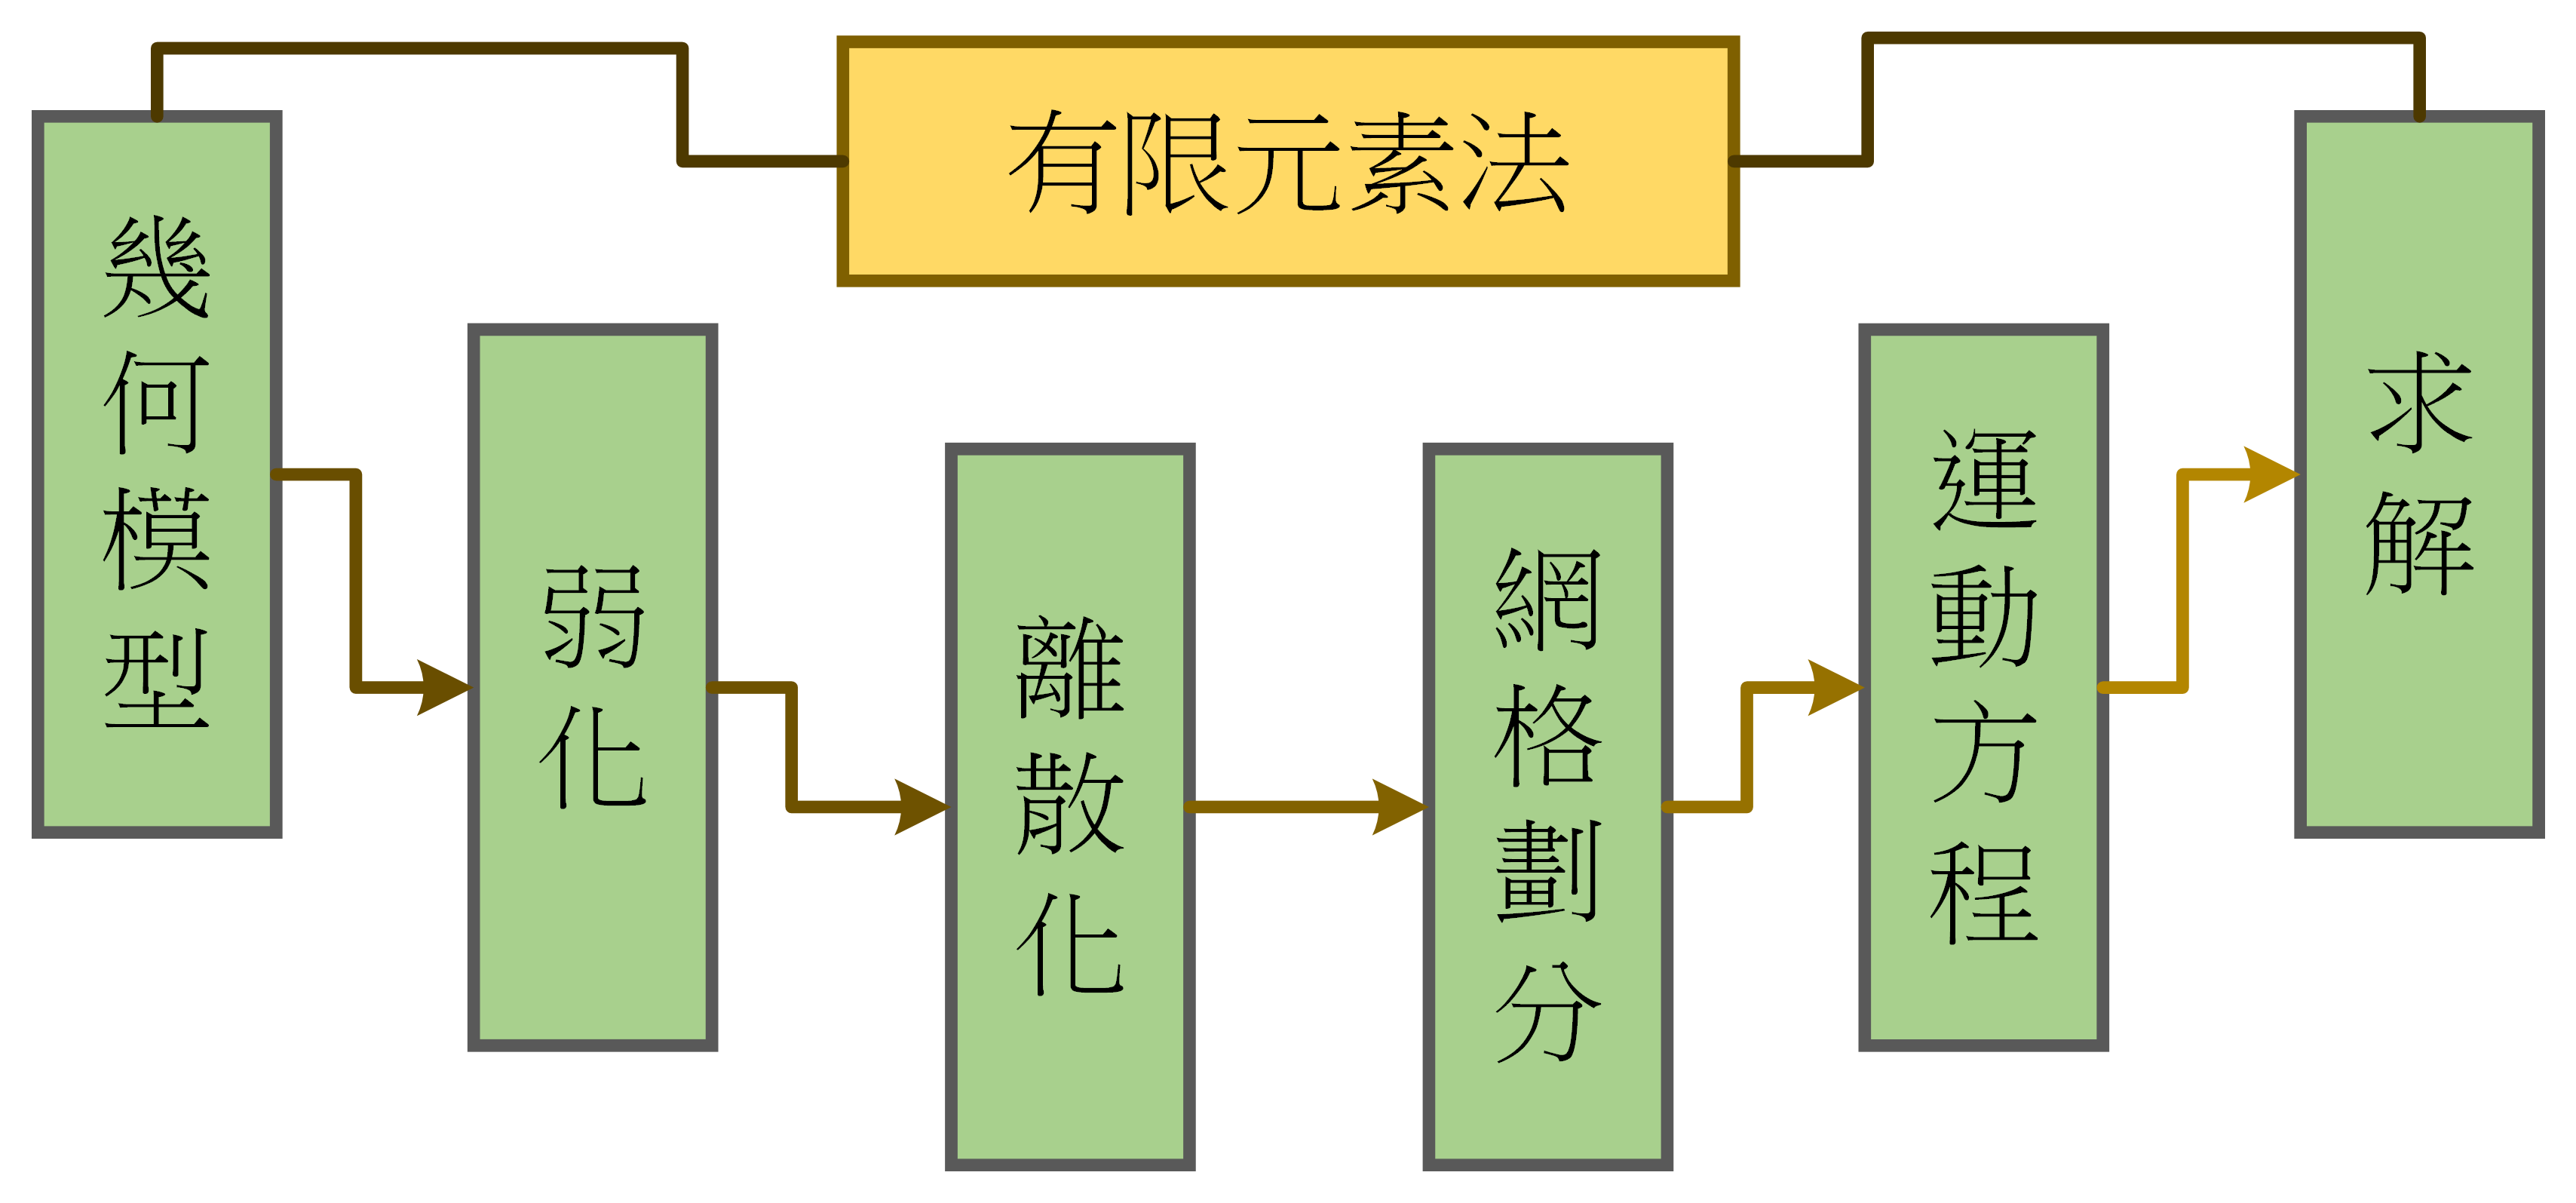
\includegraphics[width=15cm]{有限元素法分析流程}
\caption{\Large 有限元素法分析流程}\label{有限元素法分析流程}
\end{center}
\end{figure}

\begin{itemize}
\item 幾何模型:透過繪圖軟體將模型畫出,將模型以數據方式在電腦裡呈現二維或三維的外觀,便於軟體將其代入且計算。
\item 離散化及元素劃分:將物理系統或結構等連續變量通過計算轉換為數格元素的過程,對於複雜的連續變量,需先進行弱化的動作,才能進行離散化將其轉變為各個元素,此動作由分析軟體內部公式計算。
\item 導入函數並組成代數方程: 模型或問題不同,力學性質及物理方程相應的關係式(應力、應變、變形、熱傳等)也會跟著變化,因此需要根據對應的問題分別導入不同的函數,需在軟體內設定問題,讓其可以對特定問題進行求解,此動作為設計者提問,軟體負責計算。
\item 求解方程:在經過有限元素法分析後,將會在每個表面得知各元素的受力情況,設計者可以根據此數據了解到模型的受力狀態或位移及負載等相關訊息,以利於後續的設計或生產。
\end{itemize}
\newpage
